The Refbox has not changed since 2017. 


\subsubsection{Overview}

The referee of the Logistic League is a machine, which is implemented in an external component. This component is called the Referee Box (Refbox) and is implemented by the RWTH Aachen University. The Refbox communicates with the robots of both teams and the MPS Stations during a game. It manages the different phases of the game and handles the scores of each team. The manual of the Refbox is located at  \url{http://www.robocup-logistics.org/refbox}.

The Refbox did not change since the last RoboCup 2017. Therefore, this chapter summarizes the most important steps to work with the Refbox. For more detailed information, the Technical Report of 2017 \cite{TR17} is recommended.


\subsubsection{Configuration}

The Refbox is installed on the Laptop of the Robocup team in the laboratory. To run the Refbox, two programs are needed: llsf-refbox and llsf-refbox-shell. The actual Refbox program is the llsf-refbox implementation. The llsf-refbox-shell is like the name says, the graphical user interface for the Refbox.

The Referee Box can be configured via the “config.yaml” file. The most important adjustments in the file are the IP addresses. 
 
 \begin{figure}[!h]
\centering
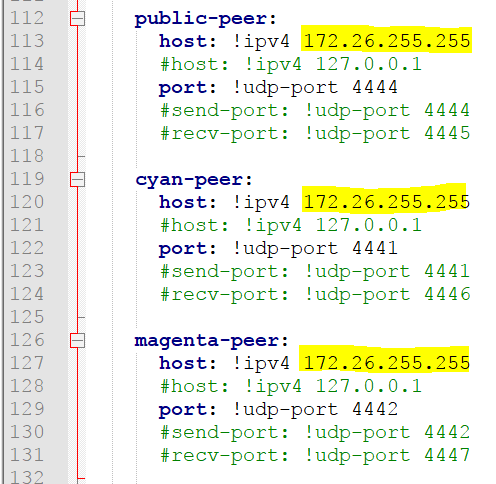
\includegraphics[]{pic/config_file_1.png}
\caption{IP adresses to modify in the config.yaml file}
\label{fig:configFile1}
\end{figure}

The other configuration part refer to the name of the team and their crypto key. 

\begin{figure}[!h]
\centering
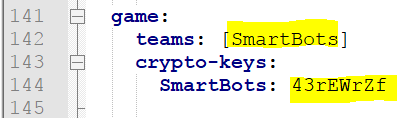
\includegraphics[]{pic/config_file_2.png}
\caption{Name and key to modify in config file}
\label{fig:configFile2}
\end{figure}

The crypto key must be the same as the key in the RefboxServer component. Therefor at the Robocup the team may adjust in the RefboxServer component the crypto key. The hosts of the game will offer a key for each team.

